%
% German documentation for 'uml2idl'.
%
% $Id$
%
\documentclass [a4paper,10pt] {scrartcl}
\usepackage{german}
\usepackage[latin1]{inputenc}
\usepackage[austrian]{babel}
%\usepackage[T1]{fontenc}


% ------------------- settings for pdf documents  ----------------------------
\expandafter\ifx\csname pdfoutput\endcsname\relax
    \usepackage[draft]{hyperref}
    \usepackage{graphicx}
    \DeclareGraphicsExtensions{.eps,.fig}
\else
    \usepackage{hyperref}
    \hypersetup{
        pdfauthor={Robert Lechner},
        pdftitle={Anleitung f{\"u}r den UML nach IDL/OCL Konverter},
        pdfsubject={Bestandteil des ccmtools Projektes},
        pdfkeywords={UML, IDL, OCL, CORBA, Komponenten, CCM}
    }
    \pdfcompresslevel=9
    \usepackage[pdftex]{graphicx}
    \DeclareGraphicsExtensions{.pdf,.png,.gif,.jpg}
\fi

\author{Robert Lechner}
\title{UML nach IDL/OCL Konverter}

\date{{\small $ $Date$ $}}

\begin{document}
\maketitle
\tableofcontents
\cleardoublepage

\section{Einleitung}
\subsection{Anwendung}
Das Paket \texttt{uml2idl} beinhaltet einen \textsf{UML}$\rightarrow$\textsf{IDL/OCL}
Konverter. Der Zweck besteht darin, Komponenten und Interfaces (\textsf{IDL}
\footnote{Interface Definition Language; Teil der CORBA-Spezifikation:\\
\url{http://www.omg.org/technology/documents/formal/corba_iiop.htm}\\
\url{http://www.omg.org/technology/documents/formal/components.htm}
}) zusammen mit der
formalen Definition der Schnittstellen (\textsf{OCL}
\footnote{Object Constraint Language; Teil der UML-Spezifikation}) in einem \textsf{UML}-Editor
zu modellieren. Der Konverter generiert daraus die f{\"u}r die \textsf{ccmtools} ben{\"o}tigten
\textsf{IDL}- und \textsf{OCL}-Dateien.
Als \textsf{UML}-Parser wird das vom Tool \texttt{dtd2java}
\footnote{Paket \texttt{dtd2java}: erzeugt Java-Modelle aus DTD-Dateien}
erzeugte Package \texttt{uml\_parser} verwendet. \\
~\\
Gestartet wird der Konverter mit dem Aufruf:
\begin{verbatim}
java uml2idl.Main UML-file IDL/OCL-prefix
\end{verbatim}
\texttt{UML-file} \dots Name der \textsf{XMI}-Datei (\textsf{UML} 1.4 -- \textsf{XMI} 1.1)
\footnote{XML Metadata Interchange: XML-Dateien zum Speichern von UML-Modellen}\\
\texttt{IDL/OCL-prefix} \dots Prefix f{\"u}r die Namen der \textsf{IDL}- und \textsf{OCL}-Dateien
\subsection{UML}
Die Komponenten und Schnittstellen werden mit Hilfe des \textsf{UML profile for CORBA}
modelliert. Als Grundlage dient die entsprechende \textsf{OMG}-Spezifikation
\footnote{UML Profile for CORBA Specification, Version 1.0, April 2002\\
UML Profile for CCM, RFP Version 2, May 2003}.\\
In Abschnitt \ref{sec:BNF} wird die Anwendung genauer erkl{\"a}rt.
\subsection{Besonderheiten}
\begin{itemize}
\item Anonyme Sequenzen und Felder bekommen einen Namen mit dem Prefix \texttt{Anonymous}
    und es wird (wie bei normalen Sequenzen und Feldern) eine \texttt{typedef}-Anweisung erzeugt.
\item Die Vorgabe der Reihenfolge mit dem \emph{tagged value} \texttt{IDLOrder} ist
    unn{\"o}tig (und wird auch nicht unterst{\"u}tzt), da die richtige Reihenfolge
    automatisch berechnet wird. Es kann aber n{\"o}tig sein, implizite Abh{\"a}ngigkeiten
    {\"u}ber eine \emph{dependency} explizit zu deklarieren.
\item Zyklische Abh{\"a}ngigkeiten k{\"o}nnen nicht aufgel{\"o}st werden!\\
    Das ist aber mit dem \emph{tagged value} \texttt{IDLOrder} ebenfalls nicht m{\"o}glich.\\
    Siehe Abschnitt \ref{sec:Cycles}.
\item \emph{fixed types} werden derzeit nicht unterst{\"u}tzt.
\end{itemize}

\newpage
\subsection{zyklische Abh{\"a}ngigkeiten}
\label{sec:Cycles}
In Abbildung \ref{fig:problem1} ist eine Abh{\"a}ngigkeit zu sehen, die nicht
aufgel{\"o}st werden kann.\\
Um diese Struktur in \textsf{IDL} zu erhalten, muss entweder \texttt{C3} oder
\texttt{C2} als "`forward declaration"' definiert werden.
Die Berechnung solcher spezieller Deklarationen ist in \texttt{uml2idl} nicht implementiert.
Es stellt sich aber die Frage, ob solche Abh{\"a}ngigkeiten nicht auf einen Designfehler hinweisen.\\
~\\
Keine Schwierigkeiten stellen die Abh{\"a}ngigkeiten in Abbildung \ref{fig:noProblem} dar.
\begin{figure}[!h]
\centerline{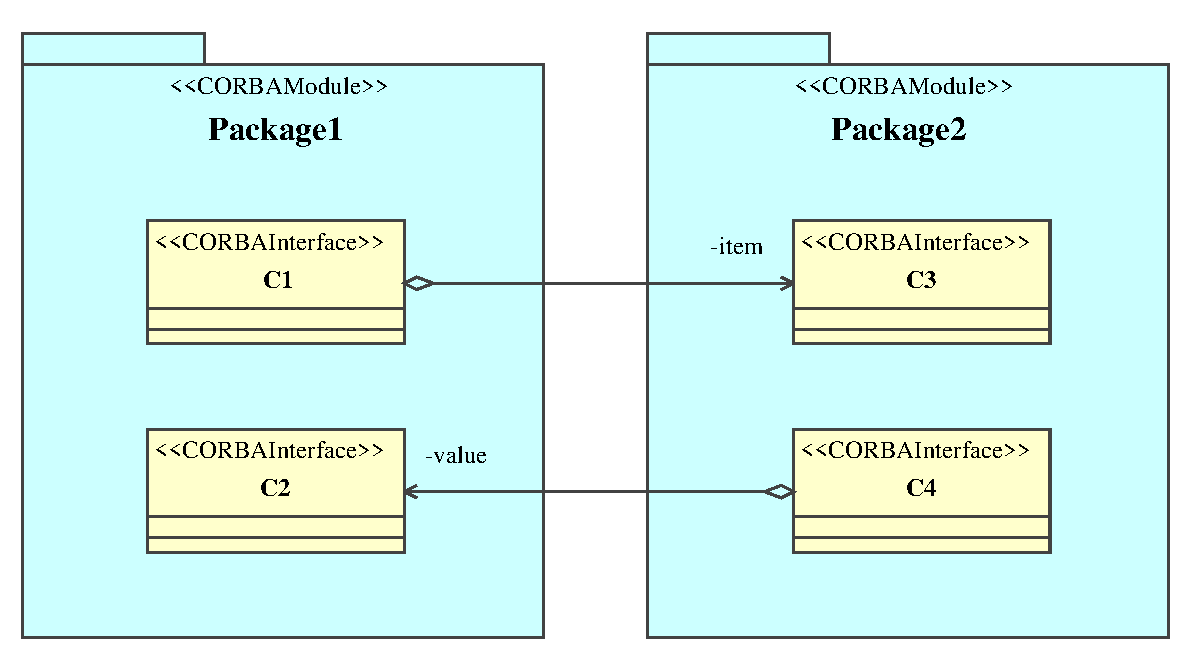
\includegraphics[width=0.8 \linewidth]{problem1}}
\caption{zyklische Abh{\"a}ngigkeit}
\label{fig:problem1}
\end{figure}
\begin{figure}[!h]
\centerline{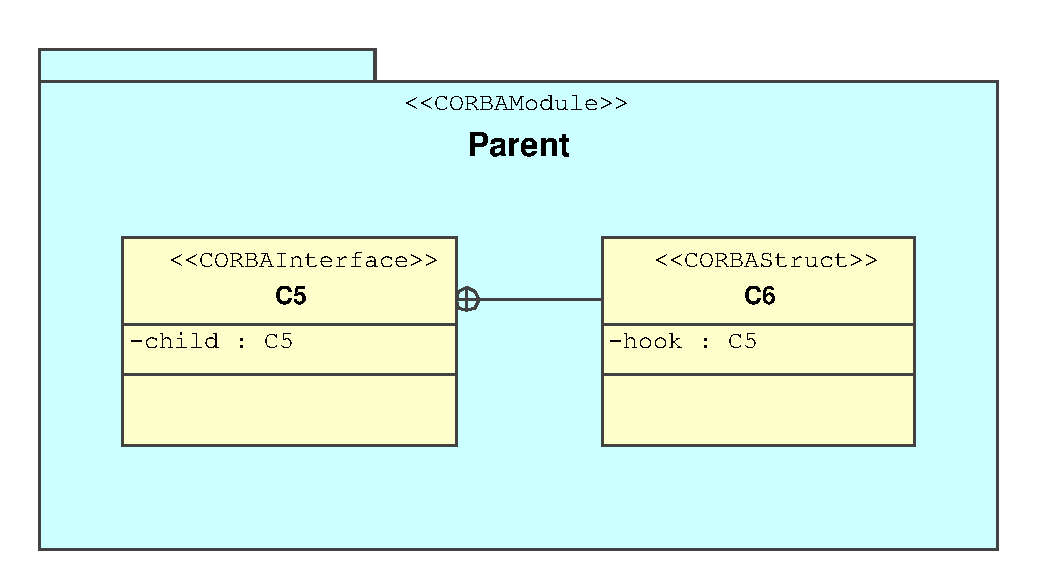
\includegraphics[width=0.8 \linewidth]{noProblem}}
\caption{Abh{\"a}ngigkeiten ohne Probleme}
\label{fig:noProblem}
\end{figure}

\cleardoublepage
\section{IDL-Grammatik und UML-Darstellung}
\label{sec:BNF}
\subsection{BNF}
\begin{verbatim}
<specification> ::= <import>* <definition>+

<import> ::= "import" (<scoped_name> | string_literal) ";"

<definition> ::= <type_dcl>
             |   <const_dcl>
             |   <except_dcl>
             |   <interface>
             |   <module>
             |   <value>
             |   <type_id_dcl>
             |   <type_prefix_dcl>
             |   <event>
             |   <component>
             |   <home_decl>

<export> ::= <type_dcl>
         |   <const_dcl>
         |   <except_dcl>
         |   <attr_dcl>
         |   <op_dcl>
         |   <type_id_dcl>
         |   <type_prefix_dcl>
\end{verbatim}

\cleardoublepage
\subsection{module}
\paragraph{IDL3}
\begin{verbatim}
<module> ::= "module" <identifier> "{" <definition>+ "};"
\end{verbatim}
\paragraph{UML}~\\
\emph{package} mit \emph{stereotype} \texttt{CORBAModule}\\
\paragraph{Beispiel}
\begin{verbatim}
module docModule {
    module Parent {
        module Child {
        };
    };
};
\end{verbatim}
\begin{figure}[!h]
\centerline{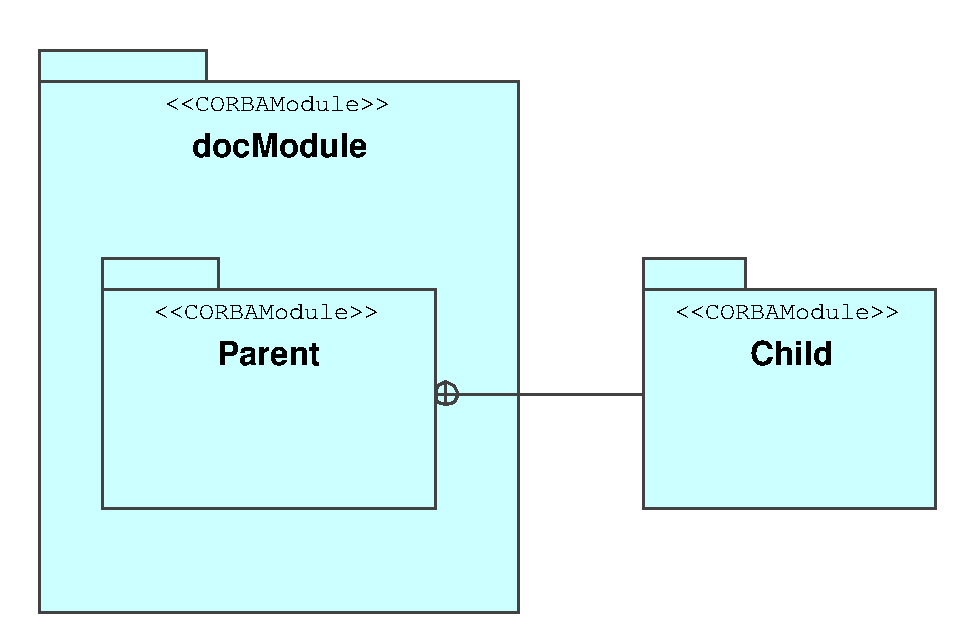
\includegraphics[width=\linewidth]{docModule}}
\caption{Zwei M{\"o}glichkeiten um Module zu verschachteln.}
\label{fig:module}
\end{figure}

\cleardoublepage
\subsection{interface}
\label{sec:interface}
\paragraph{IDL3}
\begin{verbatim}
<interface>        ::= <interface_dcl>
                   |   ["abstract" | "local"] "interface" <identifier> ";"

<interface_dcl>    ::= <interface_header> "{" <export>* "};"

<interface_header> ::= ["abstract" | "local"] "interface" <identifier>
                       [":" <interface_name> {"," <interface_name>}*]
\end{verbatim}
\paragraph{UML}~\\
\emph{class} mit \emph{stereotype} \texttt{CORBAInterface}\\
"'abstract"': abstrakte Klasse\\
"'local"': \emph{tagged value} \texttt{isLocal = TRUE}\\
Vererbung: normale Klassen-Vererbung\\
\paragraph{Beispiel}
\begin{verbatim}
module docInterface {
    local interface I1 {
    };

    abstract interface I2 {
    };

    interface I4 {
    };

    interface I3 : I2, I4 {
        struct S1 {
            long value;
        };

        attribute string myAttr;
        attribute S1 myStruct;
        long myOp(in double param);
    };
};
\end{verbatim}
\begin{figure}[!h]
\centerline{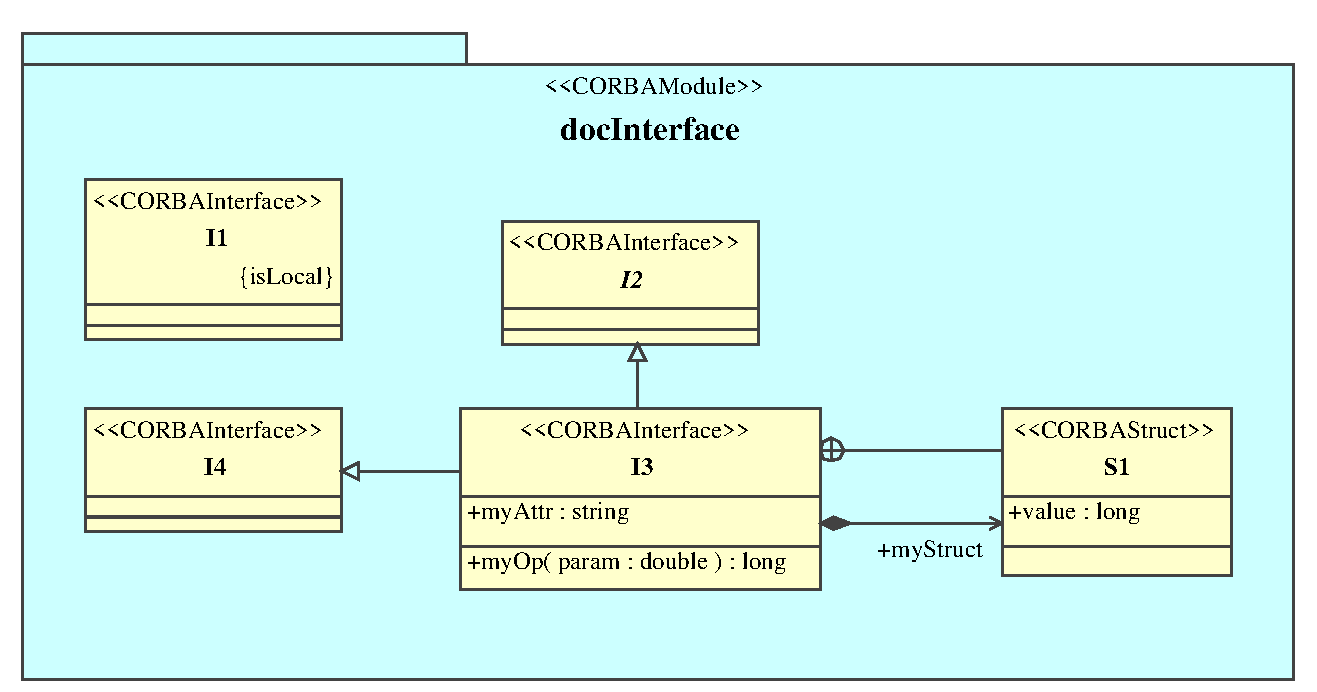
\includegraphics[width=1.2 \linewidth]{docInterface}}
\caption{UML-Klassendiagramm zu Abschnitt \ref{sec:interface}}
\label{fig:interface}
\end{figure}

\cleardoublepage
\subsection{valuetype}
\label{sec:valuetype}
\paragraph{IDL3}
\begin{verbatim}
<value>         ::= (<value_dcl> | <value_abs_dcl> | <value_box_dcl>)
                |   ["abstract"] "valuetype" <identifier> ";"

<value_box_dcl> ::= "valuetype" <identifier> <type_spec> ";"

<value_abs_dcl> ::= "abstract" "valuetype" <identifier>
                    [<value_inheritance_spec>] "{" <export>* "};"

<value_dcl>     ::= <value_header> "{" <value_element>* "};"

<value_header>  ::= ["custom"] "valuetype" <identifier>
                    [<value_inheritance_spec>]

<value_inheritance_spec> ::= [":" ["truncatable"] <value_name> {"," <value_name>}*]
                             ["supports" <interface_name> {"," <interface_name>}*]

<value_element> ::= <export> | <state_member> | <init_decl>

<state_member>  ::= ("public"|"private") <type_spec> <declarators> ";"

<init_decl>     ::= "factory" <identifier> "(" [<init_param_decls>] ")"
                    [<raises_expr>] ";"

<init_param_decls> ::= <init_param_decl> {"," <init_param_decl>}*

<init_param_decl>  ::= "in" <param_type_spec> <simple_declarator>
\end{verbatim}
\paragraph{UML}
\begin{itemize}
\item \emph{class} mit \emph{stereotype} \texttt{CORBAValue}
(Ausnahmen: "'custom"' und \emph{boxed value type})
    \begin{itemize}
    \item "'custom"': \emph{stereotype} \texttt{CORBACustomValue}
    \item \emph{boxed value type}: \emph{stereotype} \texttt{CORBABoxedValue} und Vererbung
    \end{itemize}
\item "'abstract"': abstrakte Klasse
\item Vererbung: normale Klassen-Vererbung
\item "'truncatable"': Vererbung mit \emph{stereotype} \texttt{CORBATruncatable}
\item "'supports"': Vererbung mit \emph{stereotype} \texttt{CORBAValueSupports}
\item "'factory"': \emph{operation} mit \emph{stereotype} \texttt{CORBAValueFactory}
\end{itemize}
\paragraph{Beispiel}
\begin{verbatim}
module docValuetype {
    struct Date {
        string value;
    };

    interface PrettyPrint {
        string print();
    };

    valuetype Time {
        public short hour;
        public short minute;
    };

    valuetype DateAndTime : Time supports PrettyPrint {
        private Date the_date;

        factory init(in short hr, in short min);
        Date getDate();
    };

    valuetype BoxedDate Date;
};
\end{verbatim}
\begin{figure}[!h]
\centerline{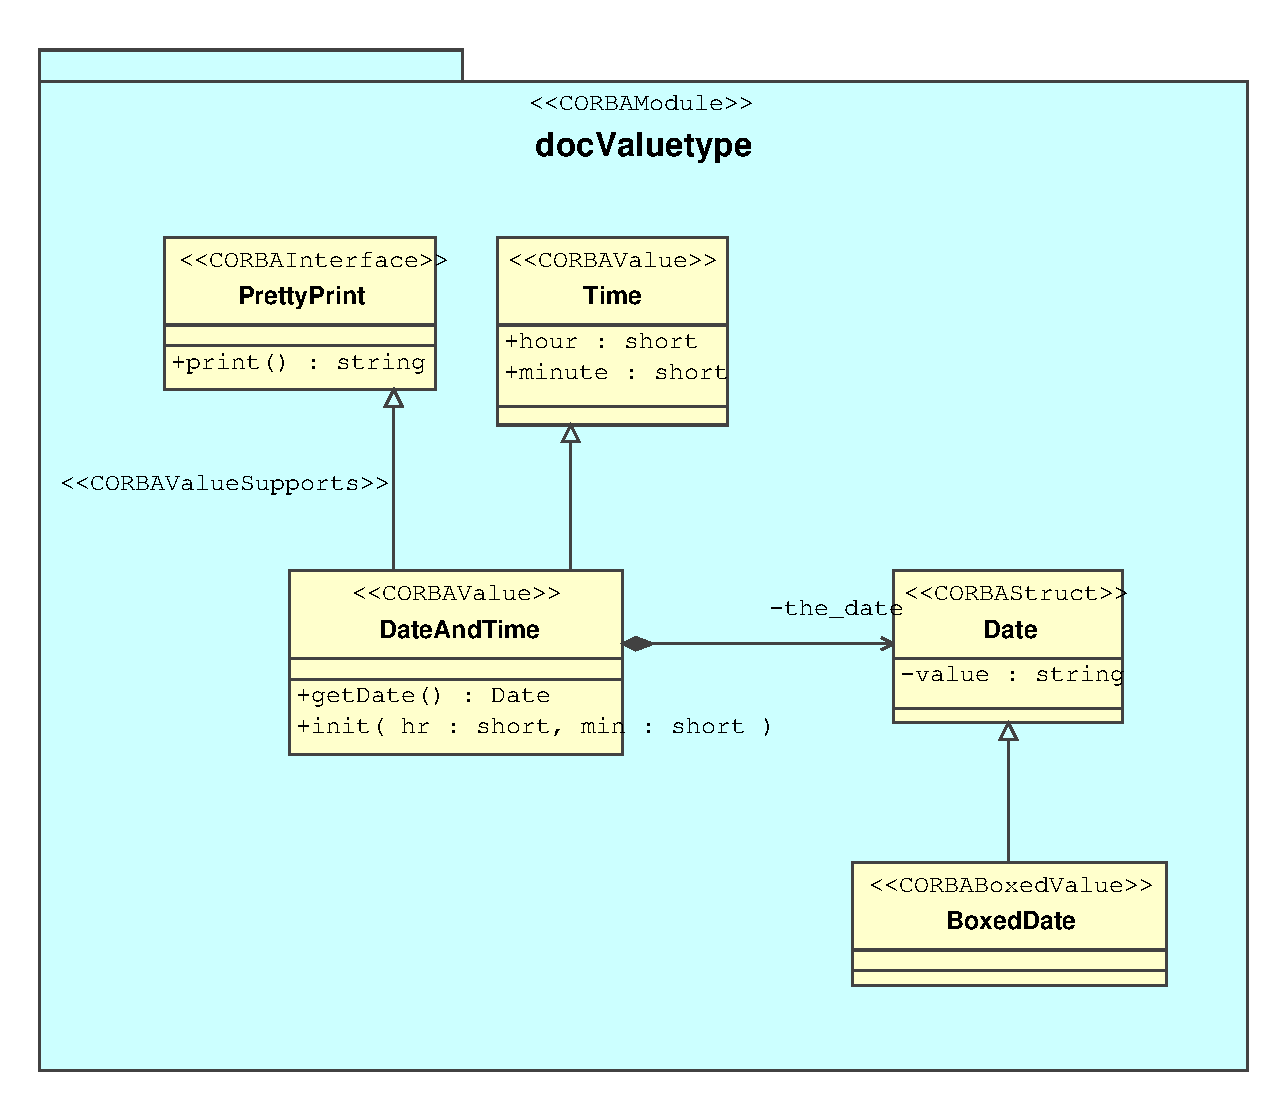
\includegraphics[width=\linewidth]{docValuetype}}
\caption{value type}
\label{fig:valuetype}
\end{figure}

\cleardoublepage
\subsection{typedef}
\paragraph{IDL3}
\begin{verbatim}
<type_dcl>  ::= "typedef" <type_spec> <declarators> ";"
            |   (<struct_type> | <union_type> | <enum_type>)
            |   "native" <identifier> ";"
            |   ("struct" |"union) <identifier> ";"

<declarators> ::= <declarator> {"," <declarators>}*

<declarator>  ::= <identifier> | <array_declarator>
\end{verbatim}
\paragraph{UML}~\\
\emph{class} oder \emph{datatype} mit \emph{stereotype} \texttt{CORBATypedef}\\
und Vererbung mit dem gew{\"u}nschten Typ.\\
\paragraph{Beispiel}
\begin{verbatim}
module docTypedef {
    interface Interface1 {
    };

    typedef Interface1 MyInterface1;

    typedef string MyString;
};
\end{verbatim}
\begin{figure}[!h]
\centerline{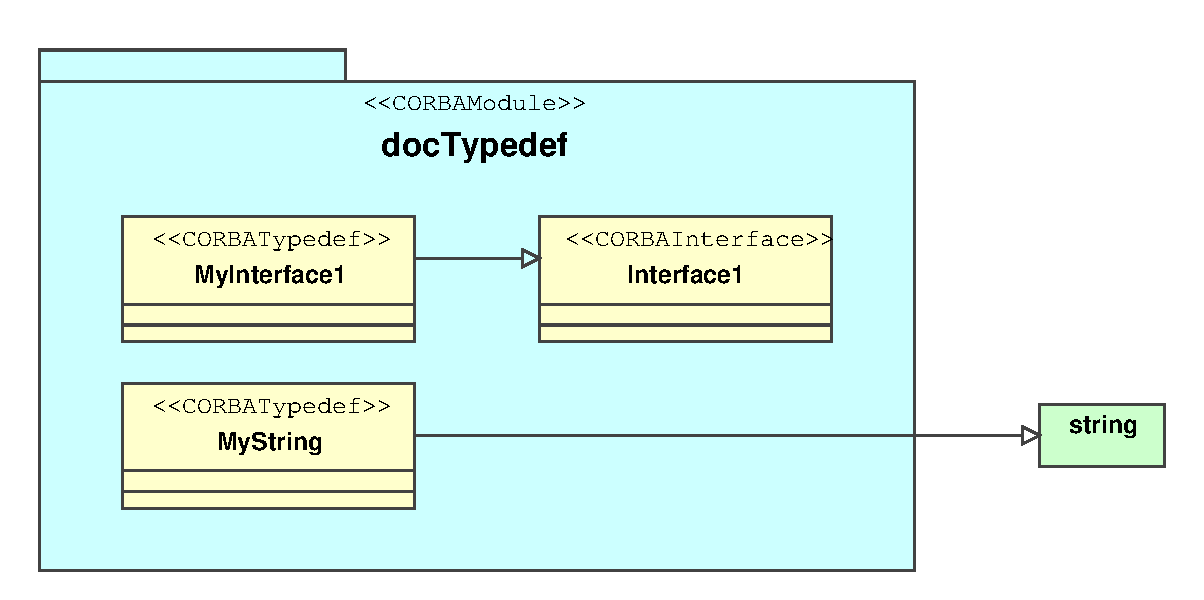
\includegraphics[width=0.9 \linewidth]{docTypedef}}
\caption{type definition}
\label{fig:typedef}
\end{figure}

\cleardoublepage
\subsection{const}
\paragraph{IDL3}
\begin{verbatim}
<const_dcl> ::= "const" <const_type> <identifier> "=" <const_exp> ";"
\end{verbatim}
\paragraph{UML}~\\
\emph{attribute} mit Stereotype \texttt{CORBAConstant}\\
\verb"<const_exp>": \emph{initial value} des Attributs\\
~\\
Globale Konstanten oder Konstanten eines Moduls:\\
\emph{class} mit \emph{stereotype} \texttt{CORBAConstants} und dem Namen \texttt{Constants};
die Konstanten werden wie oben als Attribute mit Stereotype \texttt{CORBAConstant} definiert.\\
~\\
Abh{\"a}ngigkeiten werden als einfache \emph{dependencies} dargestellt.\\
\paragraph{Beispiel}
\begin{verbatim}
module docConst {
    const short S = 3;

    interface A {
        const long L = S+20;
    };
};
\end{verbatim}
\begin{figure}[!h]
\centerline{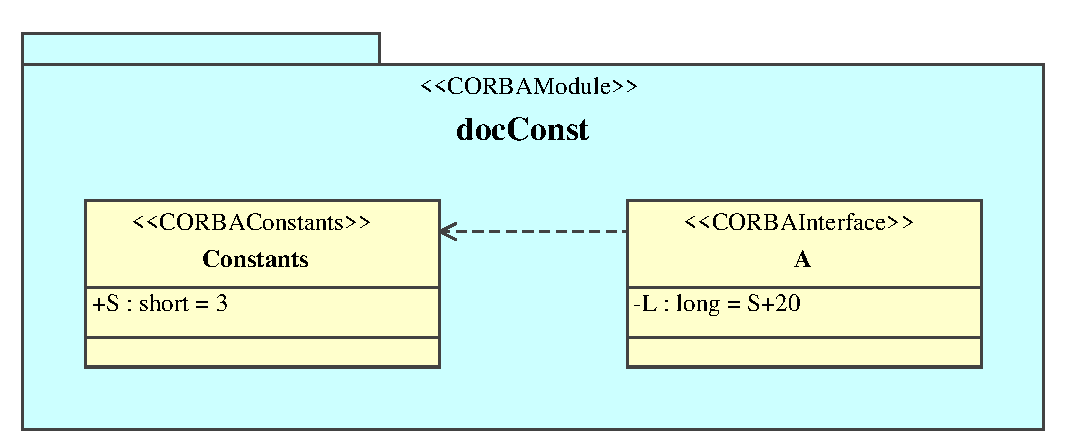
\includegraphics[width=\linewidth]{docConst}}
\caption{Konstanten mit Abh{\"a}ngigkeit}
\label{fig:const}
\end{figure}

\cleardoublepage
\subsection{struct}
\paragraph{IDL3}
\begin{verbatim}
<struct_type> ::= "struct" <identifier> "{" <member>+ "};"

<member> ::= <type_spec> <declarators> ";"
\end{verbatim}
\paragraph{UML}~\\
\emph{class} mit \emph{stereotype} \texttt{CORBAStruct}\\
\paragraph{Beispiel}
\begin{verbatim}
module docStruct {
    struct A {
        struct B {
            short k;
            long j;
        };

        string q;
        B p;
    };
};
\end{verbatim}
\begin{figure}[!h]
\centerline{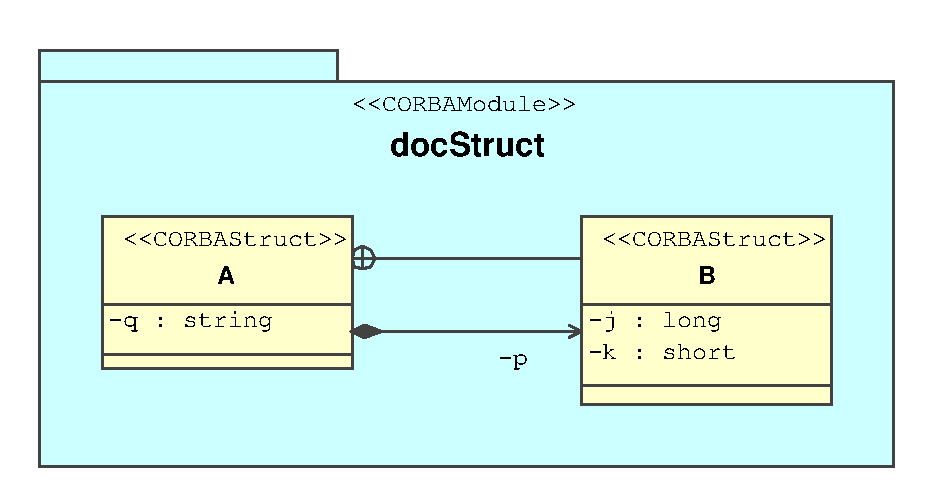
\includegraphics[width=\linewidth]{docStruct}}
\caption{zwei verschachtelte Strukturen}
\label{fig:struct}
\end{figure}

\cleardoublepage
\subsection{union}
\paragraph{IDL3}
\begin{verbatim}
<union_type> ::= "union" <identifier> "switch"
                 "(" <switch_type_spec> ")"
                 "{" <case>+ "};"

<case>       ::= <case_label>+ <type_spec> <declarator> ";"

<case_label> ::= "case" <const_exp> ":"
             |   "default:"
\end{verbatim}
\paragraph{UML}~\\
\emph{class} mit \emph{stereotype} \texttt{CORBAUnion}\\
\verb"<switch_type_spec>": \emph{association} zum Typ mit \emph{stereotype} \texttt{switchEnd}
oder Attribut mit \emph{stereotype} \texttt{switch}\\
"'case"': Attribut oder \emph{association} mit \emph{tagged value} \texttt{Case=}\emph{LabelName}\\
"'default"': Attribut oder \emph{association} mit \emph{tagged value} \texttt{Case=default}\\
\paragraph{Beispiel}
\begin{verbatim}
module docUnion {
    enum Contents {
        INTEGER_CL,
        FLOAT_CL,
        DOUBLE_CL,
        COMPLEX_CL,
        STRUCTURED_CL
    };

    union Reading switch(Contents) {
        case INTEGER_CL: long a_long;
        case FLOAT_CL: case DOUBLE_CL: double a_double;
        default: any an_any;
    };

    struct PropertyValue {
        string value;
    };

    union ValOpt switch(boolean) {
        case TRUE: PropertyValue pv;
    };
};
\end{verbatim}
\begin{figure}[!h]
\centerline{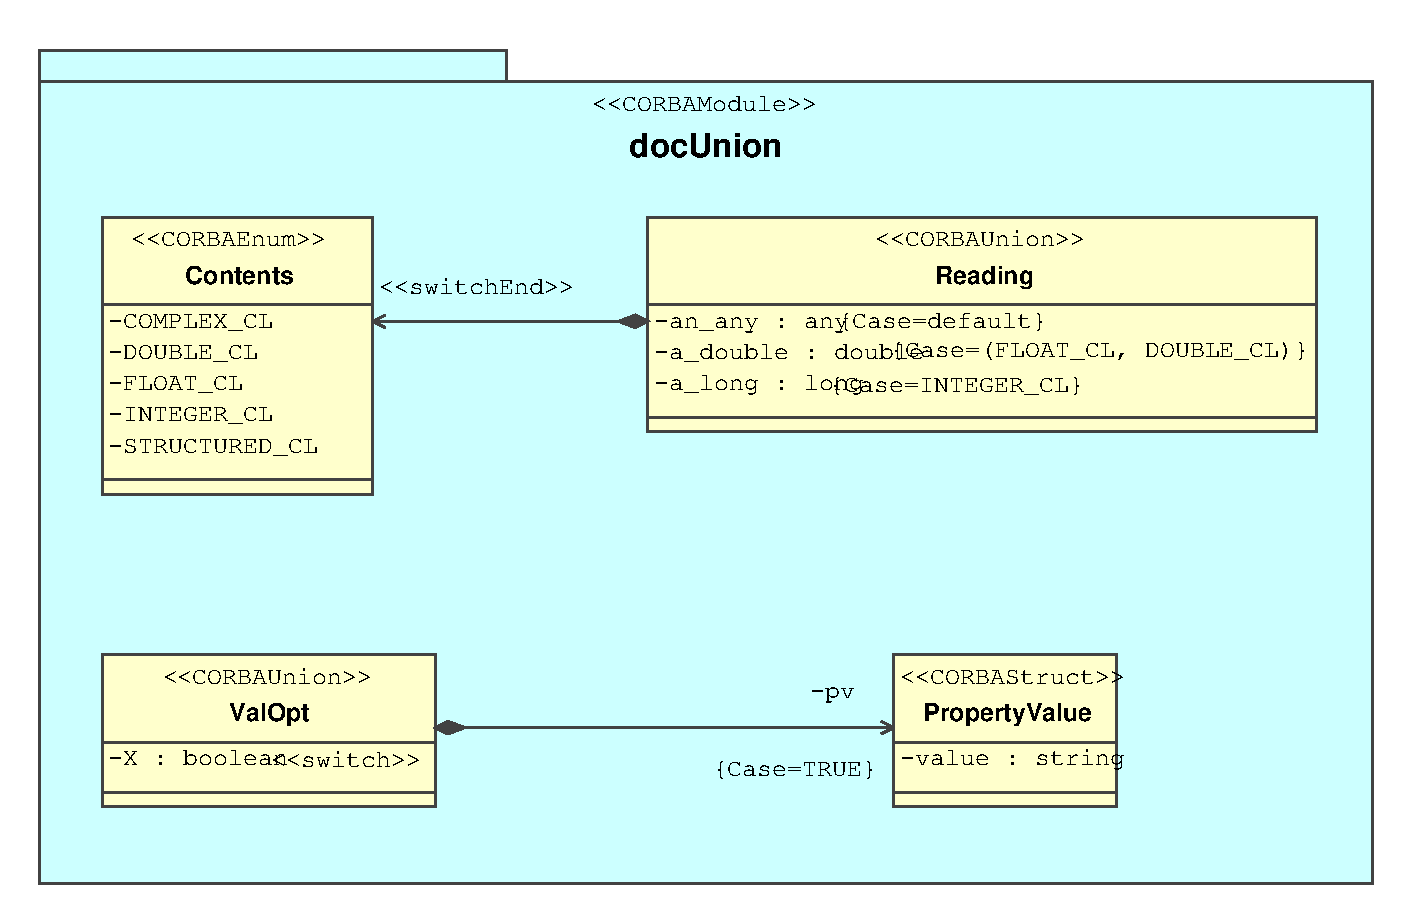
\includegraphics[width=1.2 \linewidth]{docUnion}}
\caption{union}
\label{fig:union}
\end{figure}

\cleardoublepage
\subsection{enum}
\paragraph{IDL3}
\begin{verbatim}
<enum_type> ::= "enum" <identifier> "{" <identifier> {"," <identifier>}* "};"
\end{verbatim}
\paragraph{UML}~\\
\emph{class} mit \emph{stereotype} \texttt{CORBAEnum}\\
Die Elemente sind Attribute; es wird nur der Name verwendet.\\
\paragraph{Beispiel}
\begin{verbatim}
module docEnum {
    enum Types {
        TYPE_INTEGER,
        TYPE_FLOAT,
        TYPE_COMPLEX
    };

    struct Value {
        string name;
        Types type;
    };
};
\end{verbatim}
\begin{figure}[!h]
\centerline{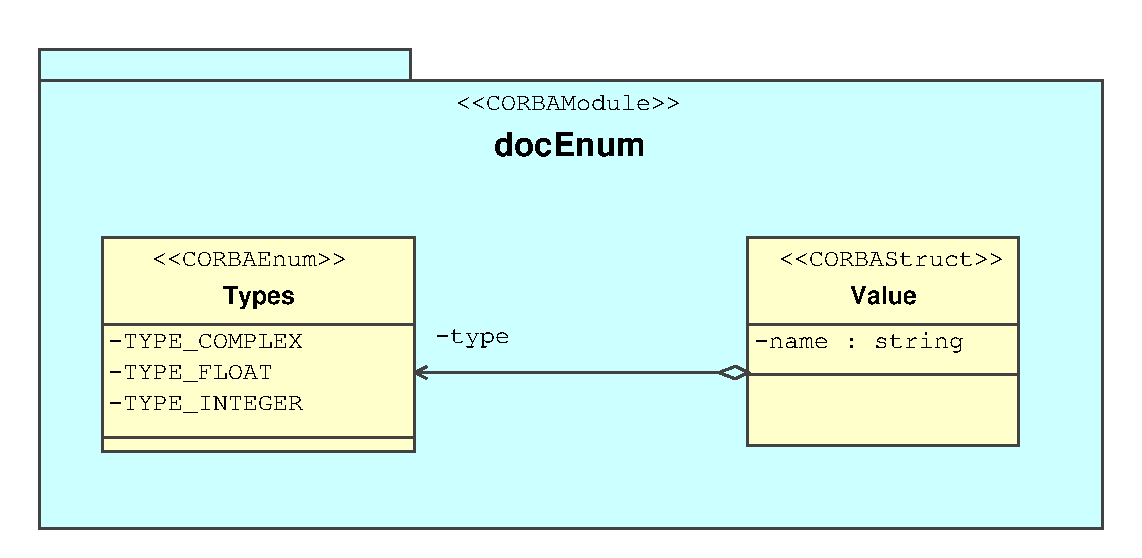
\includegraphics[width=\linewidth]{docEnum}}
\caption{enumeration}
\label{fig:enum}
\end{figure}

\cleardoublepage
\subsection{exception}
\paragraph{IDL3}
\begin{verbatim}
<except_dcl> ::= "exception" <identifier> "{" <member>* "};"

<member> ::= <type_spec> <declarators> ";"
\end{verbatim}
\paragraph{UML}~\\
\emph{class} mit \emph{stereotype} \texttt{CORBAException}\\
\paragraph{Beispiel}
\begin{verbatim}
module docException {
    interface Tex {
        exception Badness2000 {
            string err_msg;
        };

        void process_token(in string tok) raises (Badness2000);
    };
};
\end{verbatim}
\begin{figure}[!h]
\centerline{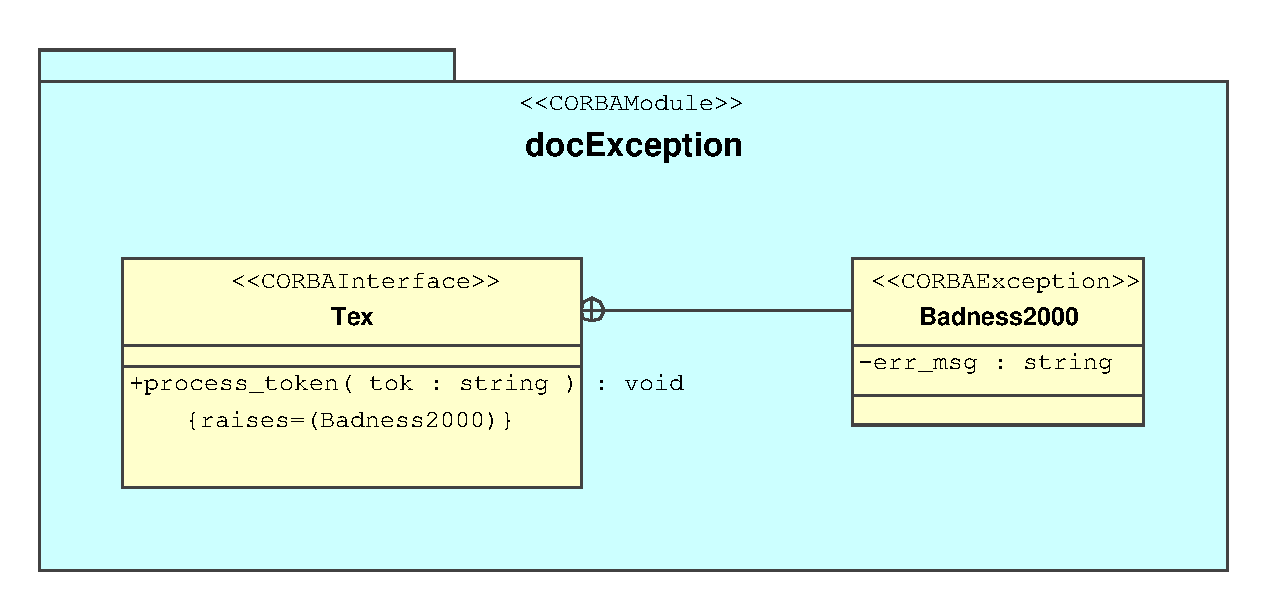
\includegraphics[width=\linewidth]{docException}}
\caption{exception}
\label{fig:exception}
\end{figure}

\cleardoublepage
\subsection{sequence}
\paragraph{IDL3}
\begin{verbatim}
<sequence_type> ::= "sequence<" <simple_type_spec> ">"
                |   "sequence<" <simple_type_spec> "," <positive_int_const> ">"
\end{verbatim}
\paragraph{UML}~\\
\emph{class} mit \emph{stereotype} \texttt{CORBASequence} oder \texttt{CORBAAnonymousSequence}\\
\emph{association} zum Typ mit \emph{qualifier} vom Typ \textbf{long} und der gew{\"u}nschten Vielfachheit\\
\paragraph{Beispiel}
\begin{verbatim}
module docSequence {
    typedef sequence< short > ShortSequence;

    typedef sequence< float > Anonymous1;

    typedef sequence< Anonymous1 > FloatMatrix;

    struct Struct1 {
        double value;
    };

    typedef sequence< Struct1 , 5 > Struct1Seq;  /* range: 0..4 */
};
\end{verbatim}
\begin{figure}[!h]
\centerline{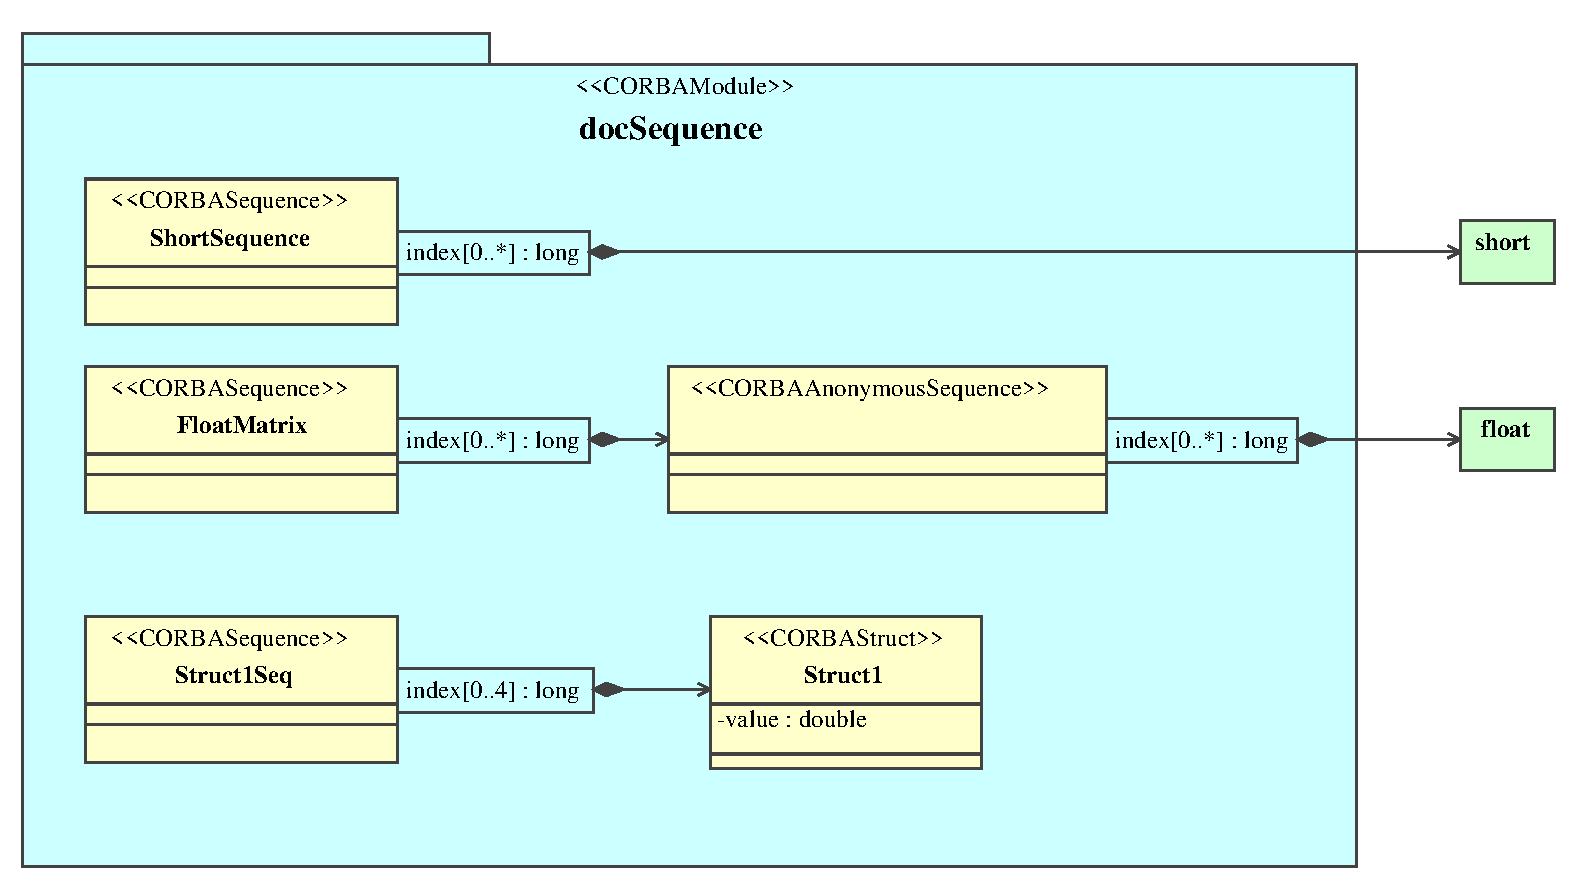
\includegraphics[width=1.2\linewidth]{docSequence}}
\caption{sequence}
\label{fig:sequence}
\end{figure}

\cleardoublepage
\subsection{array}
\paragraph{IDL3}
\begin{verbatim}
<array_declarator> ::= <identifier> <fixed_array_size>+

<fixed_array_size> ::= "[" <positive_int_const> "]"
\end{verbatim}
\paragraph{UML}~\\
\emph{class} mit \emph{stereotype} \texttt{CORBAArray} oder \texttt{CORBAAnonymousArray}\\
\emph{association} zum Typ mit \emph{qualifieres} vom Typ \textbf{long}
und den gew{\"u}nschten Vielfachheiten\\
\paragraph{Beispiel}
\begin{verbatim}
module docArray {
    struct MyStruct {
        long value;
    };

    typedef MyStruct MyArray[5][10];

    typedef MyStruct Anonymous2[4];

    struct Data1 {
        Anonymous2 field;
    };
};
\end{verbatim}
\begin{figure}[!h]
\centerline{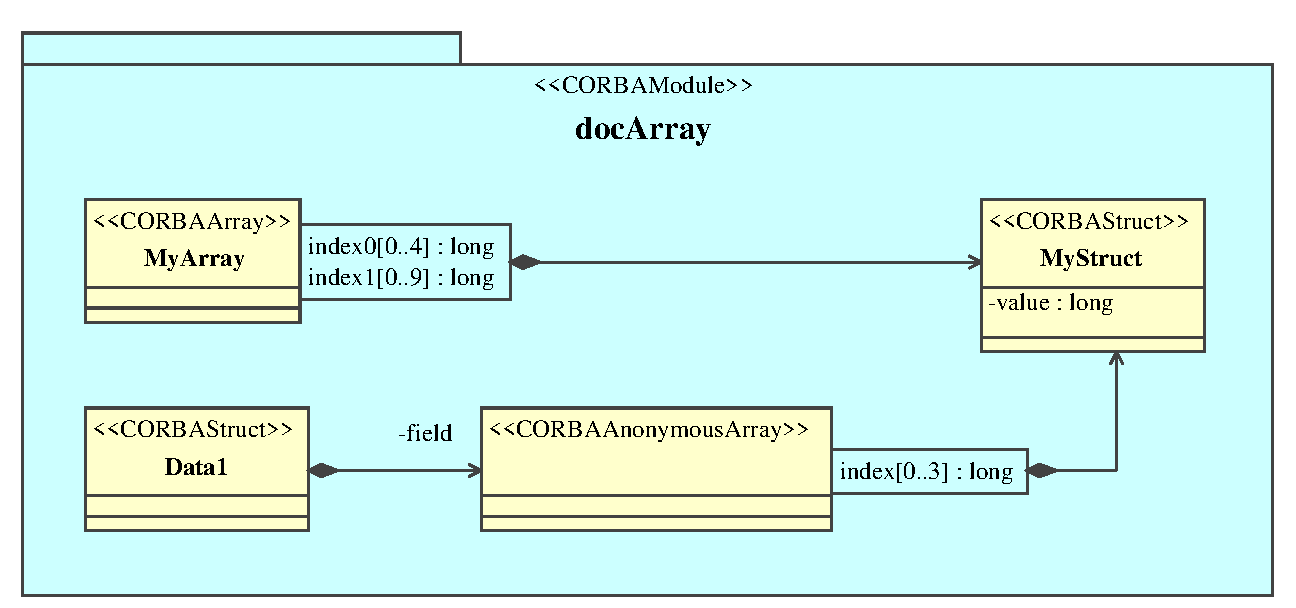
\includegraphics[width=1.2\linewidth]{docArray}}
\caption{ein- und mehrdimensionale Felder}
\label{fig:array}
\end{figure}

\cleardoublepage
\subsection{operation}
\paragraph{IDL3}
\begin{verbatim}
<op_dcl> ::= ["oneway"] <op_type_spec> <identifier> <parameter_dcls>
             [<raises_expr>] [<context_expr>] ";"

<op_type_spec>    ::= <param_type_spec> | "void"

<parameter_dcls>  ::= "(" <param_dcl> {"," <param_dcl>}* ")"
                  |   "()"

<param_dcl>       ::= ("in" | "out" | "inout")
                      <param_type_spec> <simple_declarator>

<raises_expr>  ::= "raises(" <scoped_name> {"," <scoped_name>}* ")"

<context_expr> ::= "context(" <string_literal> {"," <string_literal>}* ")"
\end{verbatim}
\paragraph{UML}~\\
UML-\emph{operation}\\
"'oneway"': \emph{stereotype} \texttt{oneway}\\
"'raises"': \emph{tagged value} \texttt{raises=}(\emph{exception1}, \emph{exception2}, \dots)\\
"'context"': \emph{tagged value} \texttt{context=}(\emph{ctx1}, \emph{ctx2}, \dots)

\cleardoublepage
\subsection{attribute}
\paragraph{IDL3}
\begin{verbatim}
<attr_dcl> ::= "attribute" <param_type_spec> <attr_declarator> ";"
           |   "readonly attribute" <param_type_spec> <readonly_attr_declarator> ";"

<attr_declarator>  ::= <simple_declarator> <attr_raises_expr>
                   |   <simple_declarator> {"," <simple_declarator>}*

<attr_raises_expr> ::= <get_excep_expr> [<set_excep_expr>]
                   |   <set_excep_expr>

<get_excep_expr>   ::= "getraises" <exception_list>

<set_excep_expr>   ::= "setraises" <exception_list>

<exception_list>   ::= "(" <scoped_name> {"," <scoped_name>}* ")"

<readonly_attr_declarator> ::= <simple_declarator> <raises_expr>
                           |   <simple_declarator> {"," <simple_declarator>}*
\end{verbatim}
\paragraph{UML}~\\
UML-\emph{attribute} oder UML-\emph{association}\\
"'readonly"' (\emph{attribute}): \emph{stereotype} \texttt{readonly}\\
"'readonly"' (\emph{association}): \emph{stereotype} \texttt{readonlyEnd} beim Typ\\
"'raises"': \emph{tagged value} \texttt{raises=}(\emph{exception1}, \emph{exception2}, \dots)\\
"'getraises"': \emph{tagged value} \texttt{getRaises=}(\emph{exception1}, \emph{exception2}, \dots)\\
"'setraises"': \emph{tagged value} \texttt{setRaises=}(\emph{exception1}, \emph{exception2}, \dots)\\
\paragraph{Beispiel}
\begin{verbatim}
module docAttribute {
    struct MyStruct {
        string value;
    };

    interface MyInterface {
        attribute long number;
        readonly attribute float myReadonlyValue;
        attribute MyStruct value1;
        readonly attribute MyStruct value2;
    };
\end{verbatim}
\newpage
\begin{verbatim}
    interface UglyInterface {
        readonly attribute long readonlyValue raises(MyException);
        attribute long value1 getraises(MyGetException) setraises(MySetException);
    };
};
\end{verbatim}
\begin{figure}[!h]
\centerline{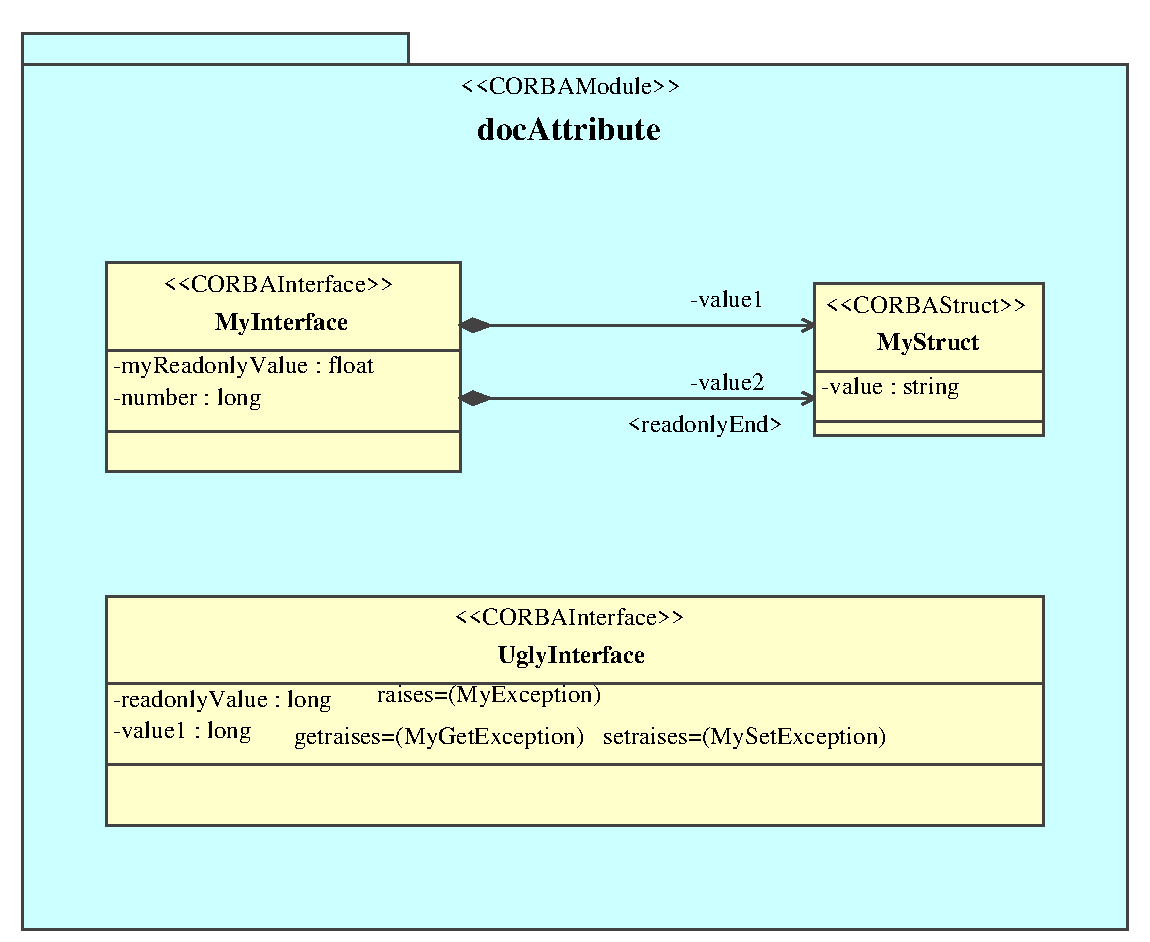
\includegraphics[width=\linewidth]{docAttribute}}
\caption{Attribute}
\label{fig:attribute}
\end{figure}

\cleardoublepage
\subsection{component}
\paragraph{IDL3}
\begin{verbatim}
<component> ::= <component_header> "{" <component_export>* "};"
            |   "component" <identifier> ";"

<component_header> ::= "component" <identifier> [":" <component_name>]
                       ["supports" <interface_name> {"," <interface_name>}*]

<component_export> ::= "provides" <interface_type> <identifier> ";"
                   |   "uses" ["multiple"] <interface_type> <identifier> ";"
                   |   "emits" <event_name> <identifier> ";"
                   |   "publishes" <event_name> <identifier> ";"
                   |   "consumes" <event_name> <identifier> ";"
                   |   <attr_dcl>

<interface_type>   ::= <scoped_name> | "Object"
\end{verbatim}
\paragraph{UML}~\\
\emph{class} mit \emph{stereotype} \texttt{CCMComponent}\\
Vererbung: normale Klassen-Vererbung\\
"'supports"': Vererbung mit \emph{stereotype} \texttt{CCMSupports}\\
"'provides"' (\textsf{facet}): \emph{association} mit \emph{stereotype} \texttt{CCMProvides}\\
"'uses"' (\textsf{receptacle}): \emph{association} mit \emph{stereotype} \texttt{CCMUses}\\
"'multiple"': Vielfachheit \texttt{1..*}\\
"'emits"': \emph{association} mit \emph{stereotype} \texttt{CCMEmits}\\
"'publishes"': \emph{association} mit \emph{stereotype} \texttt{CCMPublishes}\\
"'consumes"': \emph{association} mit \emph{stereotype} \texttt{CCMConsumes}\\
~\\
Anstelle der \emph{association} kann auch ein normales Attribut mit dem
entsprechenden \emph{stereotype} verwendet werden.
\newpage
\paragraph{Beispiel}
\begin{verbatim}
module docComponent {
    interface I1 {
    };

    interface I2 {
    };

    interface Facet1 {
    };

    component Comp1 supports I1, I2 {
        attribute long value1;
        uses Facet1 hook;
    };

    interface I3 {
    };

    interface Facet2 {
    };

    interface Facet3 {
    };

    eventtype MyEvent {
    };

    component Comp2 : Comp1 supports I3 {
        provides Facet1 facet1;
        uses Facet2 receptacle1;
        uses multiple Facet3 receptacle2;
        emits MyEvent event1;
        publishes MyEvent event2;
        consumes MyEvent event3;
    };
};
\end{verbatim}
\begin{figure}[!h]
\centerline{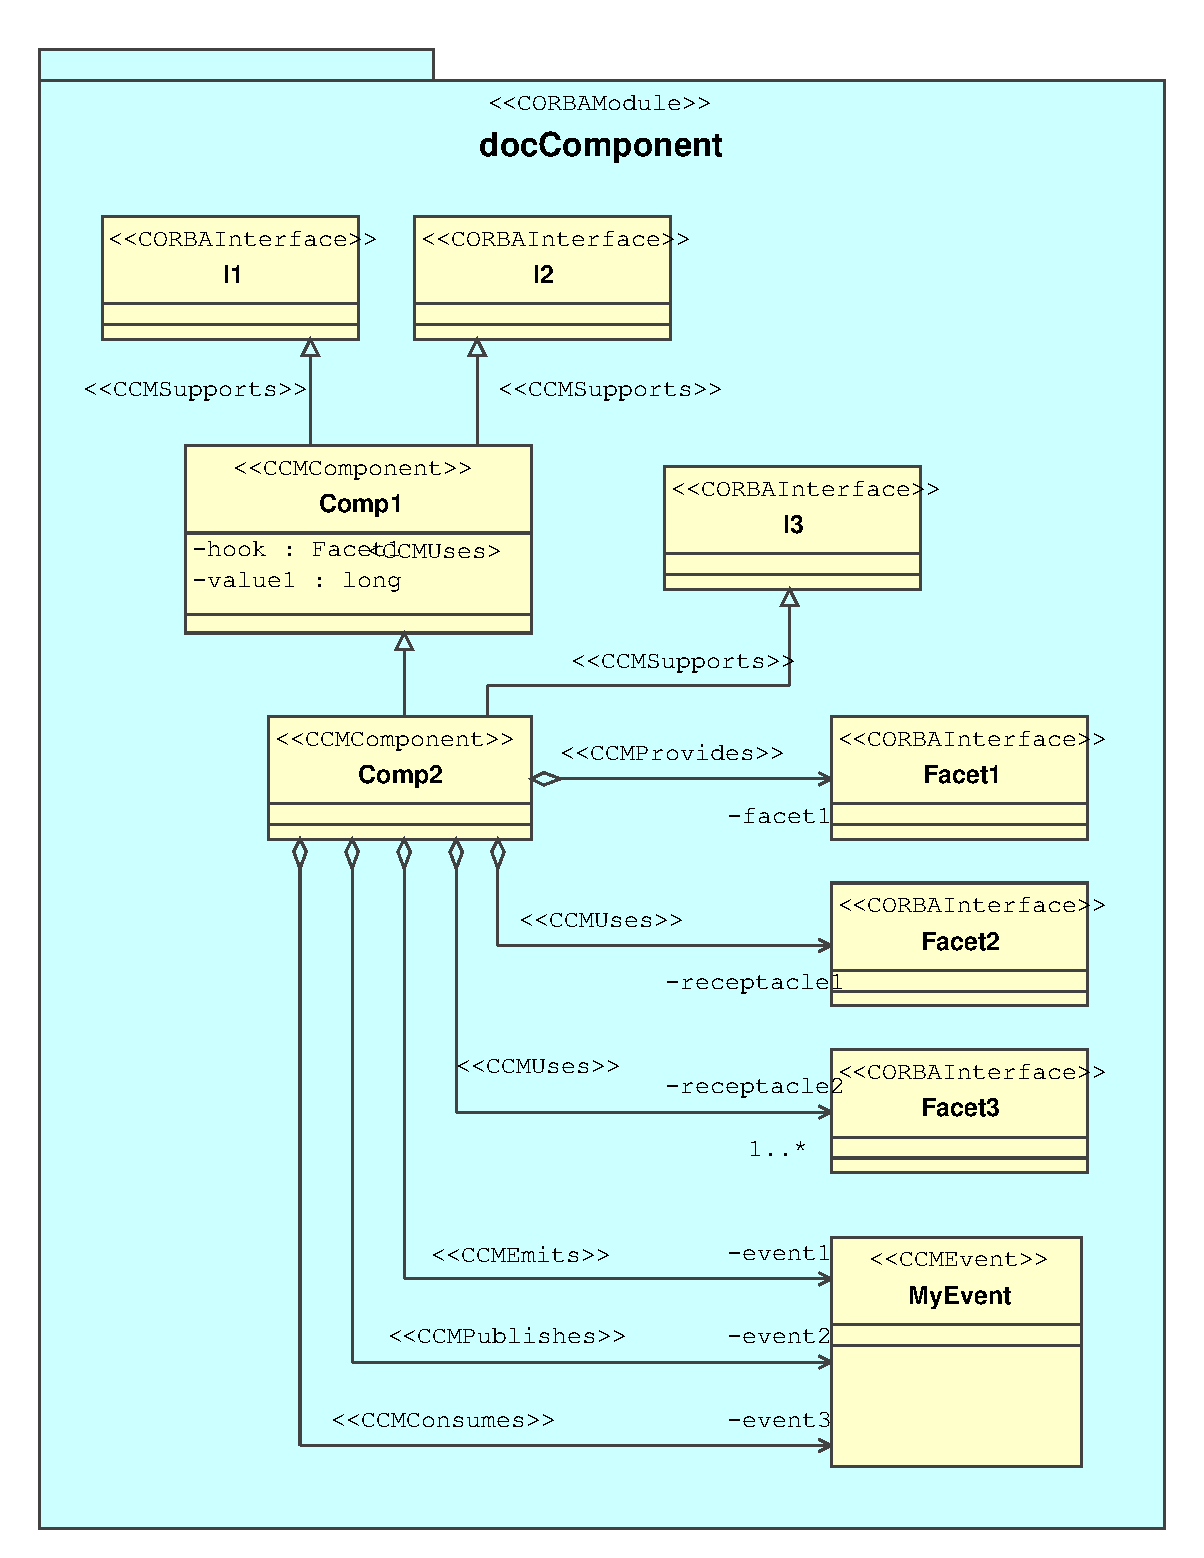
\includegraphics[width=\linewidth]{docComponent}}
\caption{Komponenten}
\label{fig:component}
\end{figure}

\cleardoublepage
\subsection{event}
\paragraph{IDL3}
\begin{verbatim}
<event> ::= (<event_dcl> | <event_abs_dcl>)
        |   ["abstract"] "eventtype" <identifier> ";"

<event_abs_dcl> ::= "abstract eventtype" <identifier> [<value_inheritance_spec>]
                    "{" <export>* "};"

<event_dcl>    ::= <event_header> "{" <value_element>* "};"

<event_header> ::= ["custom"] "eventtype" <identifier> [<value_inheritance_spec>]
\end{verbatim}
\paragraph{UML}~\\
\emph{class} mit \emph{stereotype} \texttt{CCMEvent}\\
siehe \textbf{valuetype} in Abschnitt \ref{sec:valuetype} auf Seite \pageref{sec:valuetype}\\
\paragraph{Beispiel}
~\\
\begin{minipage}{0.6 \linewidth}
\begin{verbatim}
module docEvent {
    abstract eventtype MyEvent {
    };

    eventtype Event1 : MyEvent {
    };

    eventtype Event2 : MyEvent {
    };
};
\end{verbatim}
\end{minipage}
\hfill
\begin{minipage}{0.4 \linewidth}
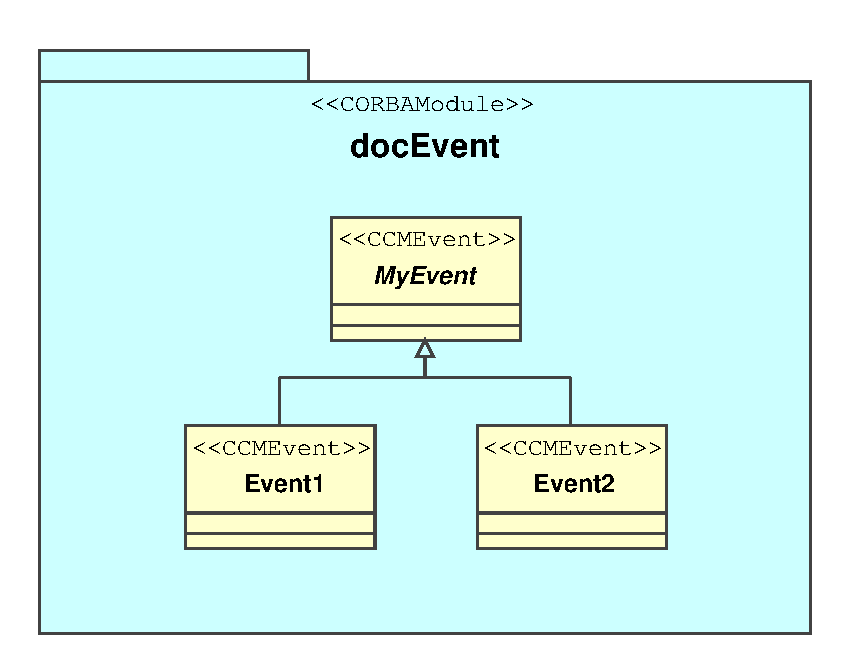
\includegraphics[width=1.4 \linewidth]{docEvent}
\end{minipage}


\cleardoublepage
\subsection{home}
\paragraph{IDL3}
\begin{verbatim}
<home_decl>   ::= <home_header> "{" <home_export>* "};"

<home_header> ::= "home" <identifier> [":" <home_name>]
                  ["supports" <interface_name> {"," <interface_name>}*]
                  "manages" <component_name>
                  ["primarykey" <scoped_name>]

<home_export> ::= <export>
              |   <factory_dcl>
              |   <finder_dcl>

<factory_dcl> ::= "factory" <identifier> "(" [<init_param_decls>] ")"
                  [<raises_expr>] ";"

<finder_dcl>  ::= "finder" <identifier> "(" [<init_param_decls>] ")"
                  [<raises_expr>] ";"
\end{verbatim}
\paragraph{UML}~\\
\emph{class} mit \emph{stereotype} \texttt{CCMHome}\\
Vererbung: normale Klassen-Vererbung\\
"'supports"': Vererbung mit \emph{stereotype} \texttt{CCMSupports}\\
"'manages"': \emph{association} mit \emph{stereotype} \texttt{CCMManages}\\
"'factory"': \emph{operation} mit \emph{stereotype} \texttt{CCMFactory}\\
"'finder"': \emph{operation} mit \emph{stereotype} \texttt{CCMFinder}\\
~\\
"'primarykey"': bei der \emph{association} (\texttt{CCMManages}) mit der Komponente entweder\\
eine \emph{association class}  mit \emph{stereotype} \texttt{CCMPrimaryKey}\\
oder ein \emph{tagged value} mit dem Namen \texttt{primarykey}\\
\paragraph{Beispiel}
\begin{verbatim}
module docHome {
    interface I1 {
    };

    component Comp1 {
        uses I1 hook;
    };
\end{verbatim}
\newpage
\begin{verbatim}
    home Home1 manages Comp1 primarykey Key {
        attribute long value;
        string print();
        finder findByName(in string name);
        factory create(in string name);
    };

    interface I2 {
    };

    home Home2 : Home1 supports I2 {
    };
};
\end{verbatim}
\begin{figure}[!h]
\centerline{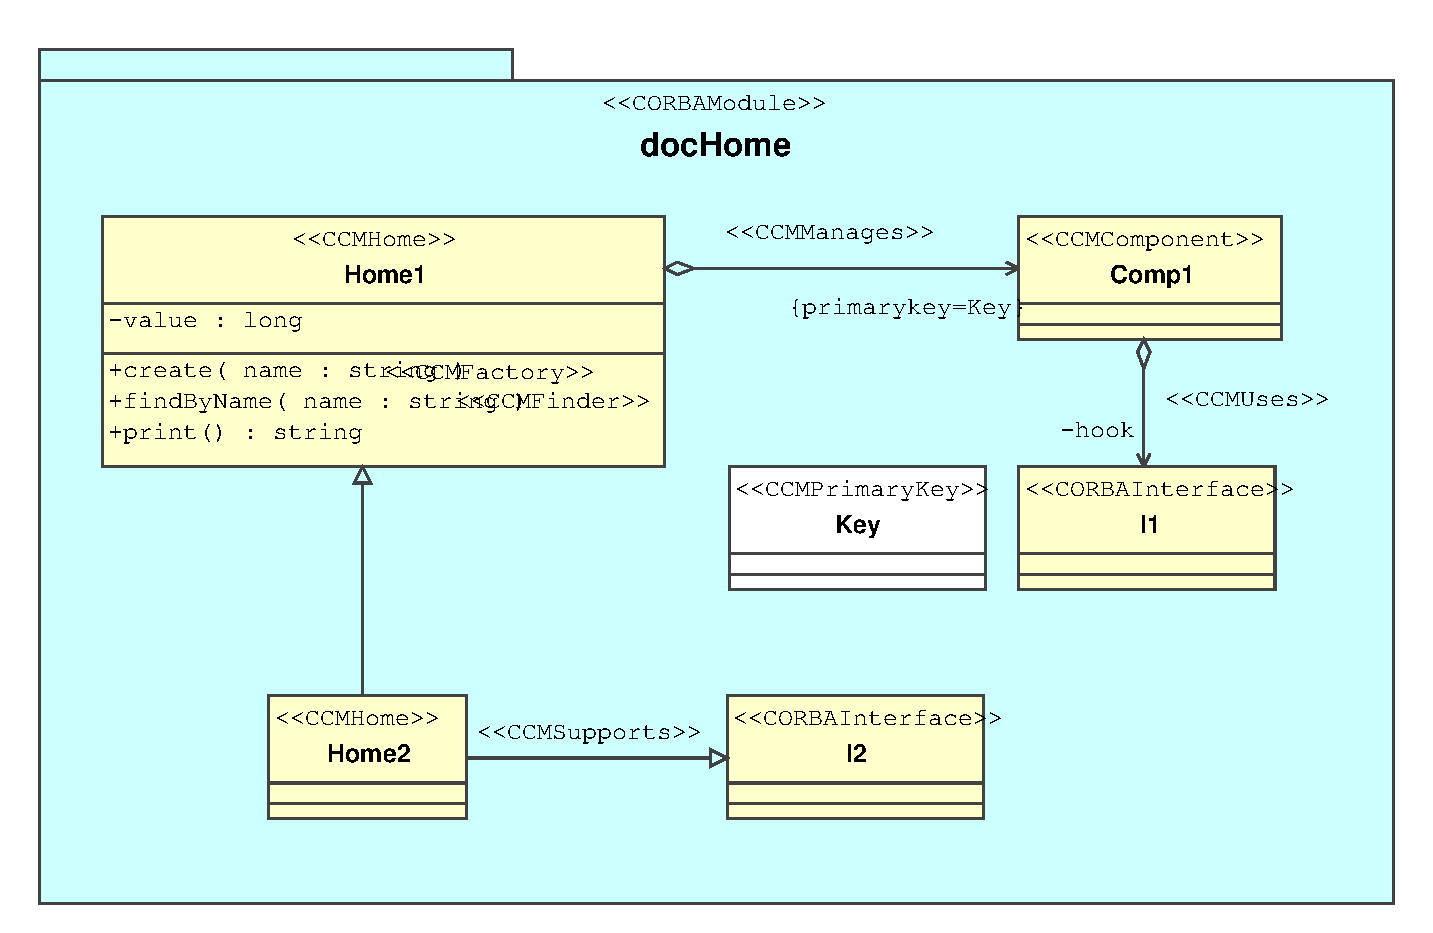
\includegraphics[width=1.2 \linewidth]{docHome}}
\caption{home}
\label{fig:home}
\end{figure}

\cleardoublepage
\section{OCL}
Die \emph{constraints} haben normalerweise folgende Form:
\begin{verbatim}
package Parent::Child
  context MyClass
    inv: company='Salomon'
    inv Name: value>0

  context MyClass::myOperation(x:Real)
    pre: x>=0
    post: result<0
endpackage
\end{verbatim}
Solche Ausdr{\"u}cke k{\"o}nnen an beliebiger Stelle definiert werden;
der Konverter schreibt sie ohne {\"A}nderung in die OCL-Datei.
Um die Eingabe zu vereinfachen, sind folgende Abk{\"u}rzungen m{\"o}glich:
\begin{itemize}
\item Pre- und Postconditions k{\"o}nnen bei der Operation oder bei einem Parameter
    ohne \texttt{package} und \texttt{context} angegeben werden:\\
    \texttt{pre: x>=0}\\
    \texttt{post check\_result: result>0}\\
\item Invarianten k{\"o}nnen bei der Klasse oder bei einem Attribut ebenfalls
    ohne \texttt{package} und \texttt{context} angegeben werden:\\
    \texttt{inv: value>=0}\\
\end{itemize}
Die fehlenden \texttt{package}- und \texttt{context}-Anweisungen werden
automatisch erzeugt.
\newpage
\textbf{Beispiel:}\\
\centerline{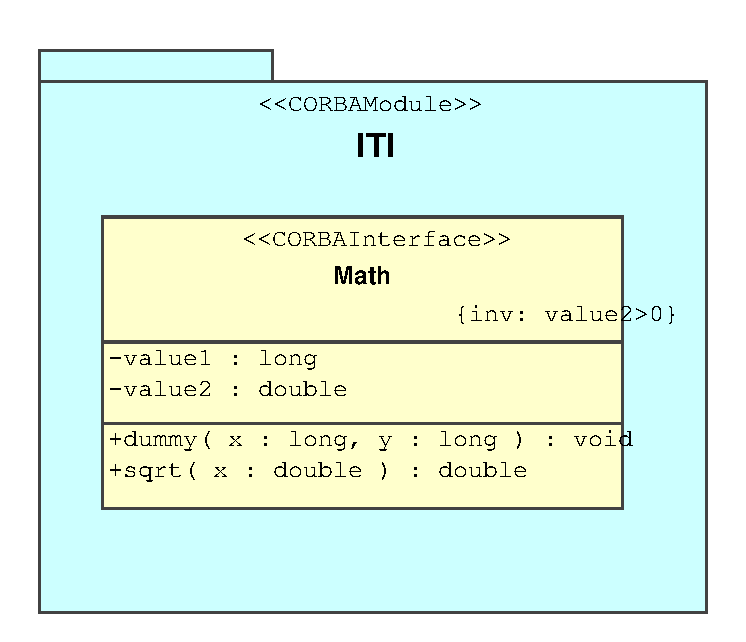
\includegraphics[width=0.6 \linewidth]{ocl1}}\\
\textbf{IDL:}
\begin{verbatim}
module ITI {
    interface Math {
        attribute long value1;
        attribute double value2;
        double sqrt(in double x);
        void dummy(in long x, in long y);
    };
};
\end{verbatim}
\textbf{OCL:}
\begin{verbatim}
package ITI
  context Math::dummy(x:Integer, y:Integer)
    pre: x>0
    pre: y>0

  context Math
    inv: value1>0
    inv: value2>0

  context Math::sqrt(x:Real)
    pre: x>=0
    post: return>=0
    post: return*return=x
endpackage
\end{verbatim}

%%---------------------------------------------------------------------------

\cleardoublepage
\section{UML-Editoren}
\subsection{MagicDraw}
\begin{itemize}
\item Es muss immer \textsf{XMI}-Version \textbf{1.1} verwendet werden.
\item Ab Version 7.x gibt es vordefinierte Profile. Diese werden nicht in
    die \textsf{XMI}-Datei kopiert. Im Editor sind sie grau hinterlegt
    und haben ein eigenes Symbol. Wird ein solches Profil ben{\"o}tigt,
    dann muss es importiert werden (rechte Maustaste -- Modul importieren).
\item Bei einem \emph{typedef} auf einen Basistyp wird als Alias f{\"u}r den
    Basistyp eine UML-Klasse mit dem Stereotype \texttt{CORBAPrimitive}
    verwendet. Der Name der Klasse ist der Name des Basistyps.
\item Der \emph{tagged value} \texttt{Case} wird bei den UML-Elementen
    \emph{Attribute} und \emph{AssociationEnd} ben{\"o}tigt.
    Falls es nicht m{\"o}glich ist beide gleichzeitig zu definieren,
    so kann f{\"u}r einen auch der Name \texttt{case} verwendet werden.
\item Der \emph{tagged value} \texttt{raises} wird bei den UML-Elementen
    \emph{Operation} und \emph{Attribute} ben{\"o}tigt.
    Falls es nicht m{\"o}glich ist beide gleichzeitig zu definieren,
    so kann f{\"u}r einen auch der Name \texttt{Raises} verwendet werden.
\item Bei der Eingabe eines Typs (z.B. f{\"u}r Attribute) ist darauf
    zu achten, dass beim Eintippen des Namens ein neuer Typ angelegt wird.
    Typen sollten daher immer ausgew{\"a}hlt werden.
\end{itemize}


\end{document}
